\documentclass[11pt]{article}

\usepackage[a4paper,margin=1in]{geometry}
\usepackage{booktabs}
\usepackage{amsmath}
\usepackage{amssymb}
\usepackage{siunitx}
\usepackage[hypertexnames=false]{hyperref}
\usepackage{graphicx}
\usepackage{float}
\usepackage[section]{placeins}

\title{RTX 5070 Reference Measurements for BMERA Gradient Throughput\\(8--256 qubits)}
\author{}
\date{\today}

\begin{document}
\maketitle

\section*{Goal}

This note summarizes the current type-1 BMERA JAX simulator measurements for
\[
  n \in \{8,16,32,64,128,256\}.
\]
For each qubit count, it reports:
\begin{itemize}
  \item measured reference data from the \texttt{*\_upd.png} throughput figures,
  \item a raw cache-only upper bound from datatype, VRAM, and bandwidth,
  \item two cross-qubit summary plots: peak throughput and fixed batch-size-64 throughput.
\end{itemize}

The measured values are the main practical result. The cache-only estimate is
kept only as an optimistic algorithmic comparison: it excludes XLA temporaries,
compiled-kernel workspaces, graph scheduling overhead, and allocator
fragmentation.

\section*{Hardware and datatype assumptions}

The simulator uses \texttt{float32} inputs and parameters. The tensor-network
intermediates therefore promote to \texttt{complex64}, i.e.
\[
  s_{\mathbb{C}} = 8\ \mathrm{bytes/complex}.
\]

The RTX 5070 constants used below are:
\[
  V = 12 \cdot 2^{30}\ \mathrm{bytes} = 12\ \mathrm{GiB},
  \qquad
  BW = 672 \times 10^9\ \mathrm{bytes/s}.
\]

\begin{table}[H]
\centering
\begin{tabular}{ll}
\toprule
Quantity & Value used in estimate \\
\midrule
GPU & GeForce RTX 5070 desktop \\
VRAM & 12 GiB \\
Memory bandwidth & 672 GB/s \\
Peak FP32 throughput & 30.87 TFLOP/s \\
BMERA type & 1 \\
Input / parameter dtype & \texttt{float32} \\
Tensor-network dtype & \texttt{complex64}, 8 bytes/element \\
\bottomrule
\end{tabular}
\end{table}

\section*{Measured reference points}

The rows below are read from the saved throughput figures whose filenames end in
\texttt{\_upd.png}. Most values are approximate figure-read values from the
plots. The previously recorded \(64\)-qubit peak throughput and peak gradient
time are kept with their exact notebook values. The \(256\)-qubit run reaches
batch \(64\), which is the largest successful batch observed for that qubit
count in the current measurements.

\begin{table}[h]
\centering
\resizebox{\textwidth}{!}{%
\begin{tabular}{rrrrrrl}
\toprule
Qubits & Largest successful batch & Peak batch & Peak throughput & Throughput at batch 64 & Peak grad time & Source \\
\midrule
8 & 4096 & 2048 & \(\approx 3.7 \times 10^5\) samples/s & \(\approx 1.0 \times 10^5\) samples/s & \(\approx 5.6\) ms & updated PNG, approximate \\
16 & 4096 & 1024 & \(\approx 1.22 \times 10^4\) samples/s & \(\approx 8.8 \times 10^3\) samples/s & \(\approx 84\) ms & updated PNG, approximate \\
32 & 1024 & 1024 & \(\approx 3.1 \times 10^3\) samples/s & \(\approx 2.55 \times 10^3\) samples/s & \(\approx 330\) ms & updated PNG, approximate \\
64 & 256 & 128 & \(981.8\) samples/s & \(\approx 8.6 \times 10^2\) samples/s & \(130.374\) ms & notebook text / updated PNG \\
128 & 128 & 128 & \(\approx 3.8 \times 10^2\) samples/s & \(\approx 3.35 \times 10^2\) samples/s & \(\approx 340\) ms & updated PNG, approximate \\
256 & 64 & 64 & \(\approx 1.2 \times 10^2\) samples/s & \(\approx 1.2 \times 10^2\) samples/s & \(\approx 530\) ms & updated PNG, approximate \\
\bottomrule
\end{tabular}%
}
\end{table}

The two aggregate views below separate the absolute best measured throughput
from the fixed-batch comparison at \(B=64\), the largest successful batch in the
current \(256\)-qubit run.

\begin{figure}[H]
\centering
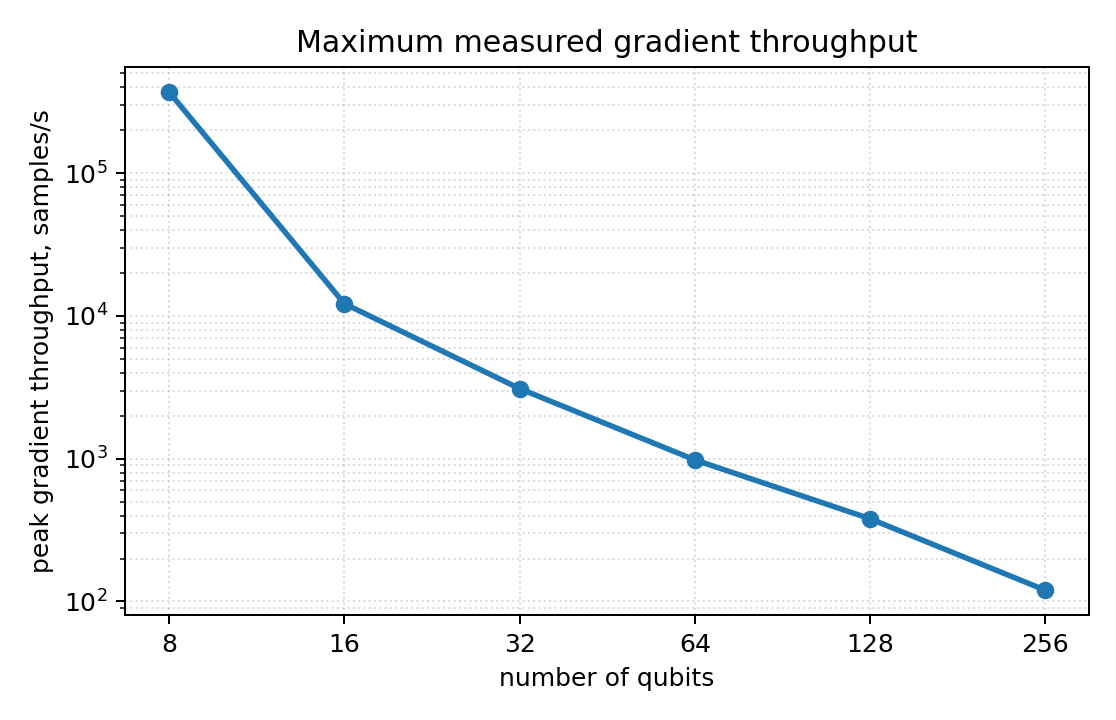
\includegraphics[width=0.72\textwidth]{max_gradient_throughput_vs_qubits.png}
\caption{Maximum measured gradient throughput versus qubit count.}
\end{figure}

\begin{figure}[H]
\centering
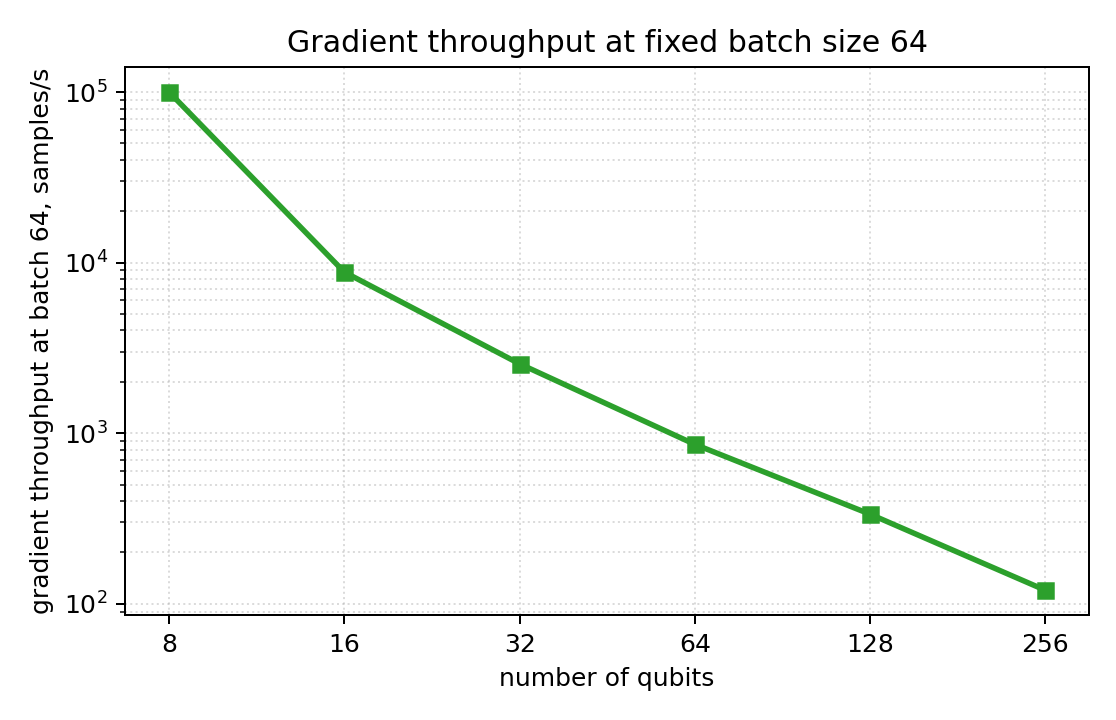
\includegraphics[width=0.72\textwidth]{batch64_gradient_throughput_vs_qubits.png}
\caption{Measured gradient throughput at fixed batch size \(64\).}
\end{figure}

\section*{Peak-throughput scaling fit}

For the peak-throughput data over \(16 \le n \le 256\), a fixed-exponent
log-space fit to
\[
  R(n) = A n^{-3/2}
\]
gives
\[
  A \approx 5.69 \times 10^5,
  \qquad
  R^2_{\log} \approx 0.989.
\]
An unconstrained log-log fit over the same points gives slope \(-1.64\), close
to the imposed \(-3/2\) scaling. Since most of the newest values are read from
figures rather than raw benchmark rows, these fit parameters should be treated as
descriptive rather than final.

\begin{table}[h]
\centering
\begin{tabular}{rrrr}
\toprule
Qubits & Measured peak throughput & \(5.69\times10^5 n^{-3/2}\) & Measured / fit \\
\midrule
16 & \(1.22 \times 10^4\) & \(8.89 \times 10^3\) & 1.37 \\
32 & \(3.10 \times 10^3\) & \(3.14 \times 10^3\) & 0.99 \\
64 & \(9.82 \times 10^2\) & \(1.11 \times 10^3\) & 0.88 \\
128 & \(3.80 \times 10^2\) & \(3.93 \times 10^2\) & 0.97 \\
256 & \(1.20 \times 10^2\) & \(1.39 \times 10^2\) & 0.86 \\
\bottomrule
\end{tabular}
\end{table}

\begin{figure}[H]
\centering
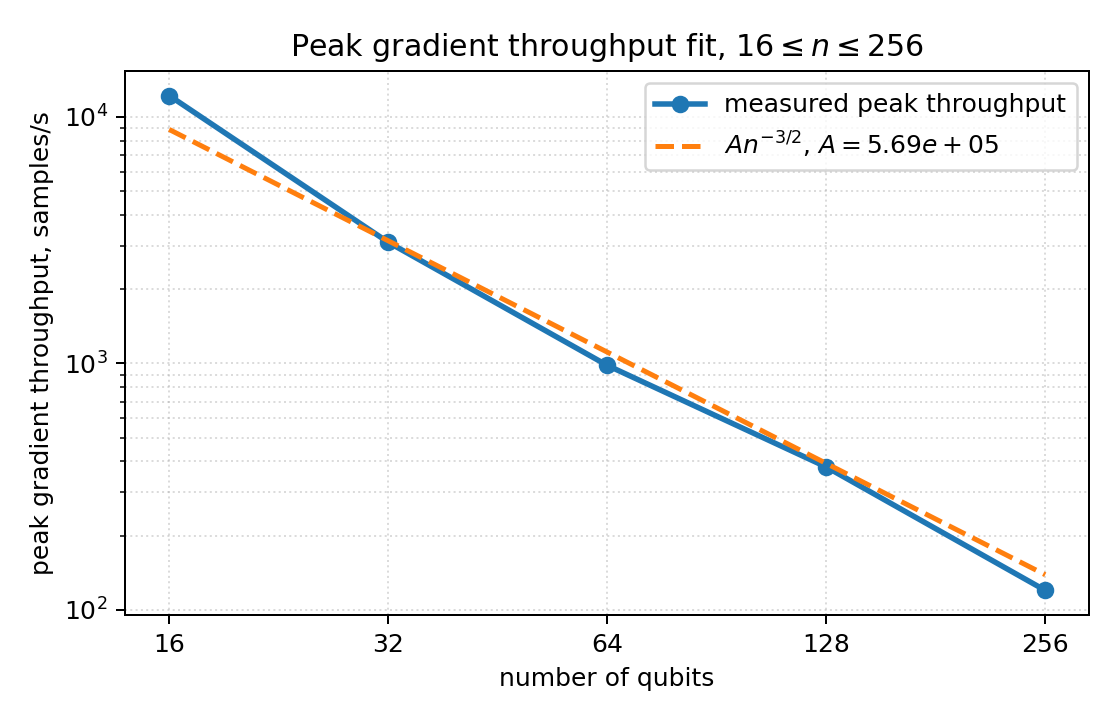
\includegraphics[width=0.72\textwidth]{peak_gradient_throughput_n_minus_3_over_2_fit.png}
\caption{Peak gradient throughput with a fixed \(n^{-3/2}\) scaling fit over \(16\)--\(256\) qubits.}
\end{figure}

The same fixed-exponent fit for the batch-size-\(64\) throughput gives
\[
  R_{64}(n) = A_{64} n^{-3/2},
  \qquad
  A_{64} \approx 4.87 \times 10^5,
  \qquad
  R^2_{\log} \approx 0.997.
\]
The unconstrained log-log slope for this fixed-batch series is \(-1.53\), which
is very close to the imposed \(-3/2\) exponent.

\begin{table}[h]
\centering
\begin{tabular}{rrrr}
\toprule
Qubits & Batch-64 throughput & \(4.87\times10^5 n^{-3/2}\) & Measured / fit \\
\midrule
16 & \(8.80 \times 10^3\) & \(7.60 \times 10^3\) & 1.16 \\
32 & \(2.55 \times 10^3\) & \(2.69 \times 10^3\) & 0.95 \\
64 & \(8.60 \times 10^2\) & \(9.50 \times 10^2\) & 0.91 \\
128 & \(3.35 \times 10^2\) & \(3.36 \times 10^2\) & 1.00 \\
256 & \(1.20 \times 10^2\) & \(1.19 \times 10^2\) & 1.01 \\
\bottomrule
\end{tabular}
\end{table}

\begin{figure}[H]
\centering
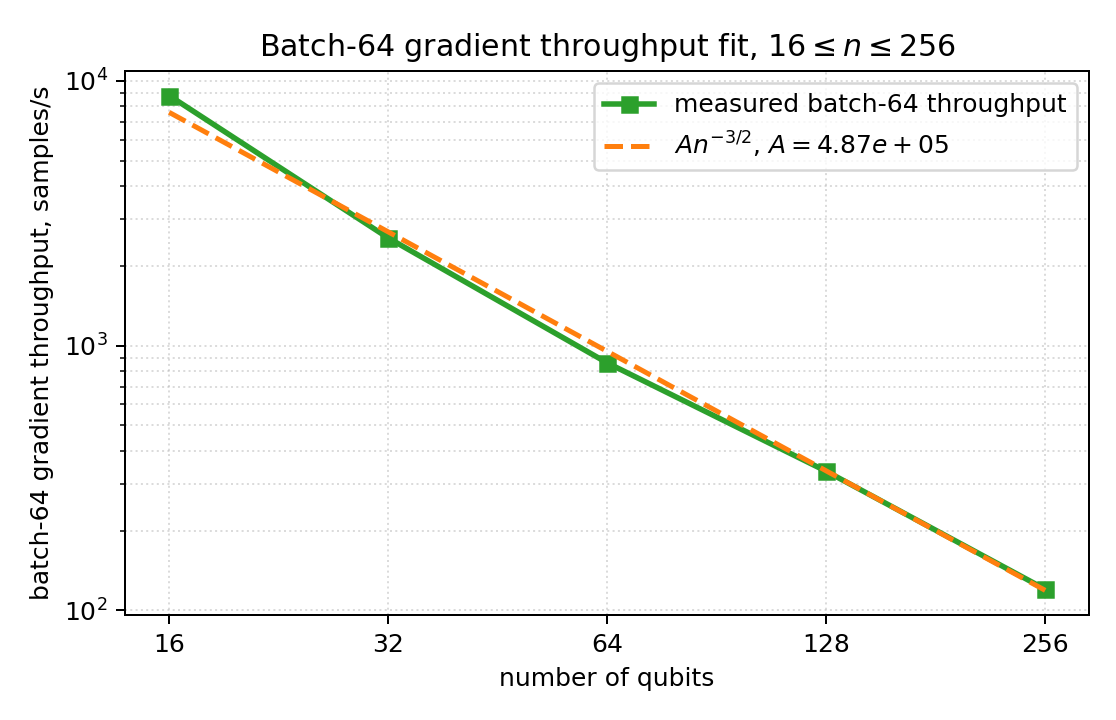
\includegraphics[width=0.72\textwidth]{batch64_gradient_throughput_n_minus_3_over_2_fit.png}
\caption{Batch-size-\(64\) gradient throughput with a fixed \(n^{-3/2}\) scaling fit over \(16\)--\(256\) qubits.}
\end{figure}

\section*{Comparison with inverse node-count scaling}

The reduced-density-node count derived below suggests another simple throughput
model: if each cached reduced-density node had approximately constant execution
cost, throughput would scale as
\[
  R(N) \propto \frac{1}{N\log_2 N}.
\]
The exact node-count formula has an additive linear correction,
\[
  C_N = N\left(2\log_2N-\frac{5}{2}\right),
\]
so we compare the previously fitted two-parameter offset model with a fixed
theory-offset model of the form
\[
  R(N) = \frac{B}{N\log_2N+\alpha N}
       = \frac{B}{N(\log_2N+\alpha)}.
\]
The figures below remove the earlier \(N^{-3/2}\) and \(1/(N\log_2N)\) curves
and show only the node-count-offset family: the requested theory-offset
\(\alpha=-2.5\) and the free-\(\alpha\) fit. Fitting the prefactor in log space
gives the following comparison.

\begin{table}[h]
\centering
\resizebox{\textwidth}{!}{%
\begin{tabular}{lrrrrr}
\toprule
Series & Model & Fitted prefactor & \(\alpha\) & \(R^2_{\log}\) & Log-RMSE \\
\midrule
Peak throughput & \(B/(N\log_2N-2.5N)\) & \(2.26 \times 10^5\) & \(-2.5\) & 0.987 & 0.180 \\
Peak throughput & \(B/(N\log_2N+\alpha N)\) & \(1.73 \times 10^5\) & \(-3.14\) & 0.997 & 0.084 \\
Batch-64 throughput & \(B_{64}/(N\log_2N-2.5N)\) & \(1.93 \times 10^5\) & \(-2.5\) & 0.997 & 0.076 \\
Batch-64 throughput & \(B_{64}/(N\log_2N+\alpha N)\) & \(1.73 \times 10^5\) & \(-2.80\) & 0.999 & 0.045 \\
\bottomrule
\end{tabular}%
}
\end{table}

\begin{figure}[H]
\centering
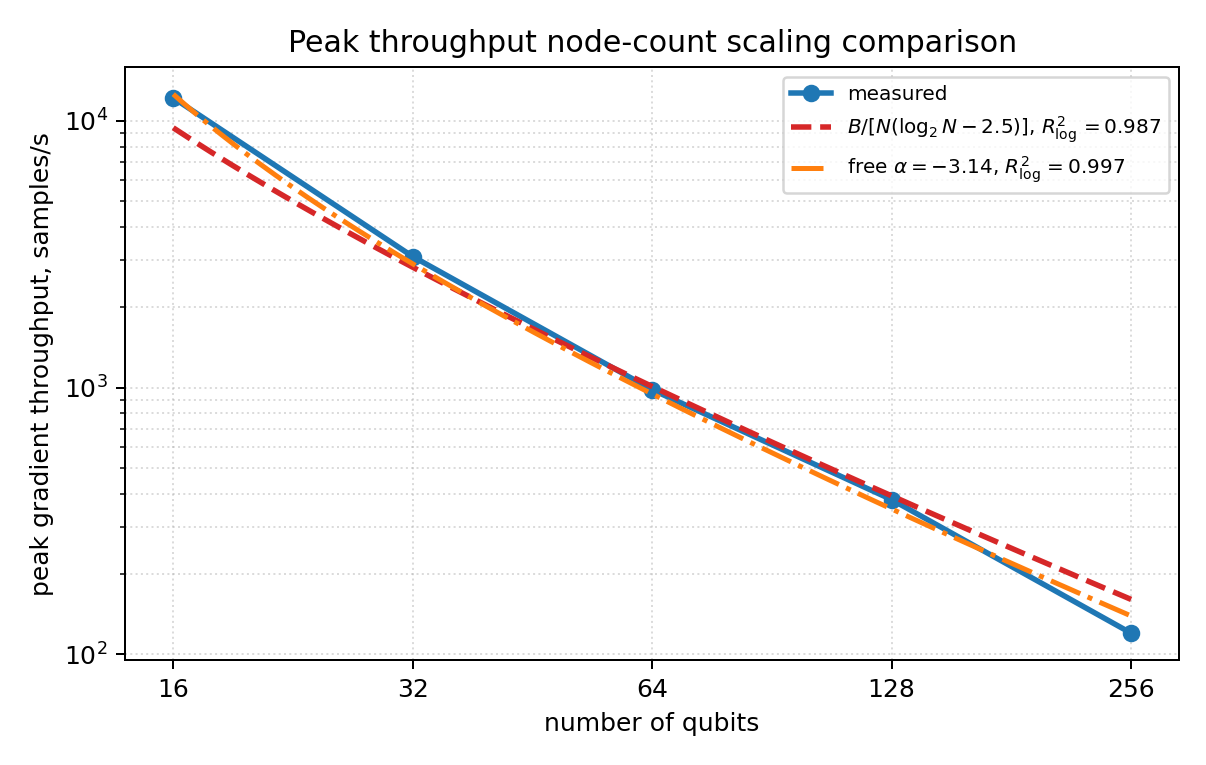
\includegraphics[width=0.72\textwidth]{peak_gradient_throughput_scaling_comparison_alpha.png}
\caption{Peak throughput compared with fixed \(\alpha=-2.5\) and free-\(\alpha\) node-count-offset fits over \(16\)--\(256\) qubits.}
\end{figure}

\begin{figure}[h]
\centering
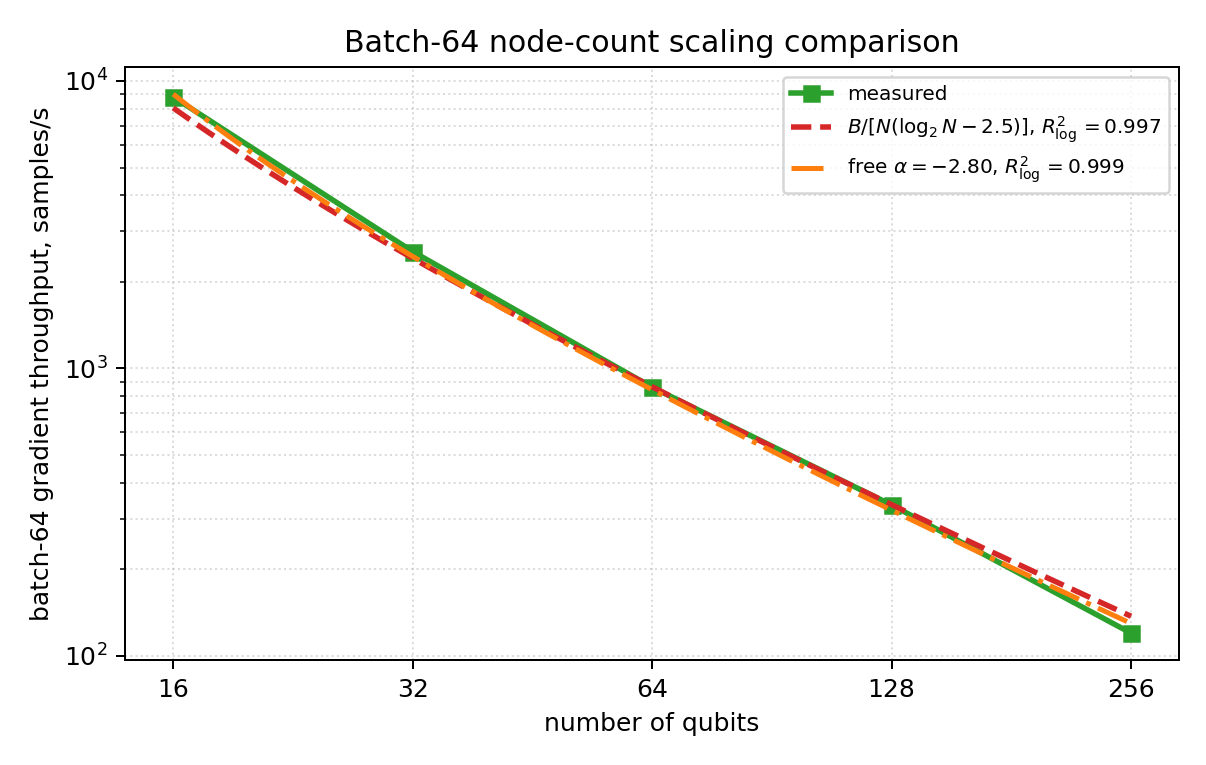
\includegraphics[width=0.72\textwidth]{batch64_gradient_throughput_scaling_comparison_alpha.png}
\caption{Batch-size-\(64\) throughput compared with fixed \(\alpha=-2.5\) and free-\(\alpha\) node-count-offset fits over \(16\)--\(256\) qubits.}
\end{figure}

The fixed \(\alpha=-2.5\) curve is close to the free-\(\alpha\) fit, especially
for the batch-size-\(64\) series. The free offset still improves the fit slightly,
but the theory-offset curve is a cleaner model because it is tied to the
negative linear correction in the reduced-density-node count. The robust
takeaway is that node-count scaling is relevant, while measured runtime also
reflects tensor rank, memory traffic, backward residuals, batching, and XLA
materialization/scheduling overhead.

\section*{Reduced-density-node scaling for all local observables}

The paper's causal-cone argument gives \(O(\log N)\) reduced density matrices
for one fixed local observable in the translation-invariant case, and
\(O(N)\) work for one local observable when all gates are distinct. In the
current simulator, the forward pass computes all \(N\) one-site \(Z\)
expectation values at once and caches shared reduced density matrices between
overlapping causal cones. The resulting node count is therefore larger than the
single-observable count, but still scales only as \(O(N\log N)\).

Let \(C_N\) be the number of non-empty reduced-density tensors in the shared
contraction plan for all one-site observables on \(N=2^T\) qubits. For
\(N\ge 8\), the plan has the recurrence
\[
  C_N = 2 C_{N/2} + 2N,
  \qquad
  C_8 = 28.
\]
Solving this recurrence gives
\[
  C_N = N\left(2\log_2 N - \frac{5}{2}\right),
  \qquad N\ge 8.
\]
Thus the number of cached reduced density matrices per qubit grows only
logarithmically,
\[
  \frac{C_N}{N} = 2\log_2 N - \frac{5}{2}.
\]

The decomposition of the current plan count is also useful for interpreting
memory and compilation cost:
\[
  C_N
  =
  \underbrace{N}_{\text{input one-qubit densities}}
  +
  \underbrace{\frac{N}{2}}_{\text{first entangling layer}}
  +
  \underbrace{N\left(\log_2 N-\frac{9}{4}\right)}_{\text{pre-green reduced states}}
  +
  \underbrace{N\left(\log_2 N-\frac{7}{4}\right)}_{\text{post-green reduced states}}.
\]
The tensor ranks remain bounded by the local causal-cone width; for the current
all-observable plan, the maximum density-tensor rank is \(12\), corresponding to
at most six active qubits in an intermediate reduced density matrix.

\begin{table}[h]
\centering
\begin{tabular}{rrrrr}
\toprule
Qubits & \(\log_2 N\) & Plan nodes \(C_N\) & Formula \(N(2\log_2N-5/2)\) & Nodes/qubit \\
\midrule
8 & 3 & 28 & 28 & 3.5 \\
16 & 4 & 88 & 88 & 5.5 \\
32 & 5 & 240 & 240 & 7.5 \\
64 & 6 & 608 & 608 & 9.5 \\
128 & 7 & 1,472 & 1,472 & 11.5 \\
256 & 8 & 3,456 & 3,456 & 13.5 \\
\bottomrule
\end{tabular}
\end{table}

This node-count scaling explains why steady-state execution can remain
polynomial and causal-cone-local while XLA compilation becomes heavy at larger
\(N\): the compiler sees thousands of statically unrolled reduced-density update
nodes for the all-observable gradient graph.

\section*{Per-sample cache sizes}

Using \texttt{cache\_profile(...)} for type-1 BMERA with \texttt{float32}
inputs/parameters, the stored forward cache per sample is:

\begin{table}[h]
\centering
\begin{tabular}{rrr}
\toprule
Qubits & \(S_{\mathrm{cache}}\) [bytes/sample] & \(S_{\mathrm{cache}}\) [MiB/sample] \\
\midrule
8 & 21,248 & 0.0203 \\
16 & 340,480 & 0.3247 \\
32 & 1,276,928 & 1.2178 \\
64 & 3,745,792 & 3.5723 \\
128 & 9,875,456 & 9.4180 \\
256 & 24,518,656 & 23.3828 \\
\bottomrule
\end{tabular}
\end{table}

\section*{Raw cache-only theory}

If the only memory cost were the explicitly stored BMERA cache, the memory and
bandwidth roofs would be
\[
  B_{\mathrm{cache}}(n) = \left\lfloor \frac{V}{S_{\mathrm{cache}}(n)} \right\rfloor,
  \qquad
  R_{\mathrm{cache}}(n) = \frac{BW}{S_{\mathrm{cache}}(n)}.
\]

\begin{table}[h]
\centering
\begin{tabular}{rrrr}
\toprule
Qubits & Cache-only batch roof & Cache-only throughput roof & Interpretation \\
\midrule
8 & 606,405 & \(3.16 \times 10^7\) samples/s & purely optimistic \\
16 & 37,843 & \(1.97 \times 10^6\) samples/s & purely optimistic \\
32 & 10,090 & \(5.26 \times 10^5\) samples/s & purely optimistic \\
64 & 3,439 & \(1.79 \times 10^5\) samples/s & purely optimistic \\
128 & 1,304 & \(6.80 \times 10^4\) samples/s & purely optimistic \\
256 & 525 & \(2.74 \times 10^4\) samples/s & purely optimistic \\
\bottomrule
\end{tabular}
\end{table}

These values are not practical current-kernel limits. They ignore temporary
tensors, XLA workspaces, graph scheduling overhead, and allocator fragmentation.

\section*{Summary result}

\begin{table}[h]
\centering
\resizebox{\textwidth}{!}{%
\begin{tabular}{rrrrrr}
\toprule
Qubits & Measured largest batch & Peak throughput & Batch-64 throughput & Cache bytes/sample & Cache-only batch roof \\
\midrule
8 & 4096 & \(\approx 3.7 \times 10^5\) & \(\approx 1.0 \times 10^5\) & 21,248 & 606,405 \\
16 & 4096 & \(\approx 1.22 \times 10^4\) & \(\approx 8.8 \times 10^3\) & 340,480 & 37,843 \\
32 & 1024 & \(\approx 3.1 \times 10^3\) & \(\approx 2.55 \times 10^3\) & 1,276,928 & 10,090 \\
64 & 256 & \(981.8\) & \(\approx 8.6 \times 10^2\) & 3,745,792 & 3,439 \\
128 & 128 & \(\approx 3.8 \times 10^2\) & \(\approx 3.35 \times 10^2\) & 9,875,456 & 1,304 \\
256 & 64 & \(\approx 1.2 \times 10^2\) & \(\approx 1.2 \times 10^2\) & 24,518,656 & 525 \\
\bottomrule
\end{tabular}%
}
\end{table}

The measurements are the best practical summary for the current code path. The
cache-only numbers remain far above the measured results and should be
interpreted as optimistic algorithmic lower bounds on memory footprint rather
than realistic throughput targets.

For the updated run, the most important large-\(n\) result is
\[
  \boxed{B_{\mathrm{largest}}(256)=64,\qquad B_{\mathrm{peak}}(256)=64,\qquad R_{\mathrm{measured}}(256)\approx 1.2\times 10^2\ \mathrm{samples/s}.}
\]

\section*{Trainability on synthetic fixed-information tasks}

Section 7 of the notebook benchmarks trainability on four binary synthetic
datasets: moons, circles, XOR, and parity. This is a fixed-information control:
the informative feature dimension is held fixed while the model input is padded
from 8 to 16 qubits. Each configuration uses three random repeats, and the table
below reports the best repeat selected by validation accuracy, breaking ties by
validation MSE. Training used full gradient batches from the throughput sweep
rather than microbatch accumulation.

\begin{table}[h]
\centering
\resizebox{\textwidth}{!}{%
\begin{tabular}{llrrrrrr}
\toprule
Dataset & Optimizer & Qubits & Repeat & Validation accuracy & Test accuracy & Validation MSE & Test MSE \\
\midrule
moons & SGD & 8 & 1 & 0.887 & 0.878 & 0.3387 & 0.3374 \\
moons & Adam & 8 & 1 & 0.887 & 0.878 & 0.3303 & 0.3306 \\
moons & SGD & 16 & 1 & 0.887 & 0.878 & 0.3380 & 0.3367 \\
moons & Adam & 16 & 0 & 0.890 & 0.877 & 0.3266 & 0.3267 \\
circles & SGD & 8 & 2 & 0.755 & 0.760 & 0.8659 & 0.8656 \\
circles & Adam & 8 & 1 & 1.000 & 1.000 & 0.0497 & 0.0510 \\
circles & SGD & 16 & 1 & 0.769 & 0.770 & 0.8313 & 0.8307 \\
circles & Adam & 16 & 1 & 1.000 & 1.000 & 0.0502 & 0.0513 \\
xor & SGD & 8 & 1 & 0.974 & 0.963 & 0.5243 & 0.5160 \\
xor & Adam & 8 & 2 & 0.959 & 0.946 & 0.4258 & 0.4214 \\
xor & SGD & 16 & 1 & 0.970 & 0.955 & 0.6384 & 0.6293 \\
xor & Adam & 16 & 1 & 0.966 & 0.956 & 0.4247 & 0.4208 \\
parity & SGD & 8 & 1 & 0.511 & 0.504 & 1.0007 & 0.9997 \\
parity & Adam & 8 & 0 & 1.000 & 1.000 & 0.4038 & 0.4043 \\
parity & SGD & 16 & 0 & 0.496 & 0.501 & 1.0002 & 0.9999 \\
parity & Adam & 16 & 2 & 1.000 & 1.000 & 0.3124 & 0.3150 \\
\bottomrule
\end{tabular}%
}
\end{table}

\begin{figure}[h]
\centering
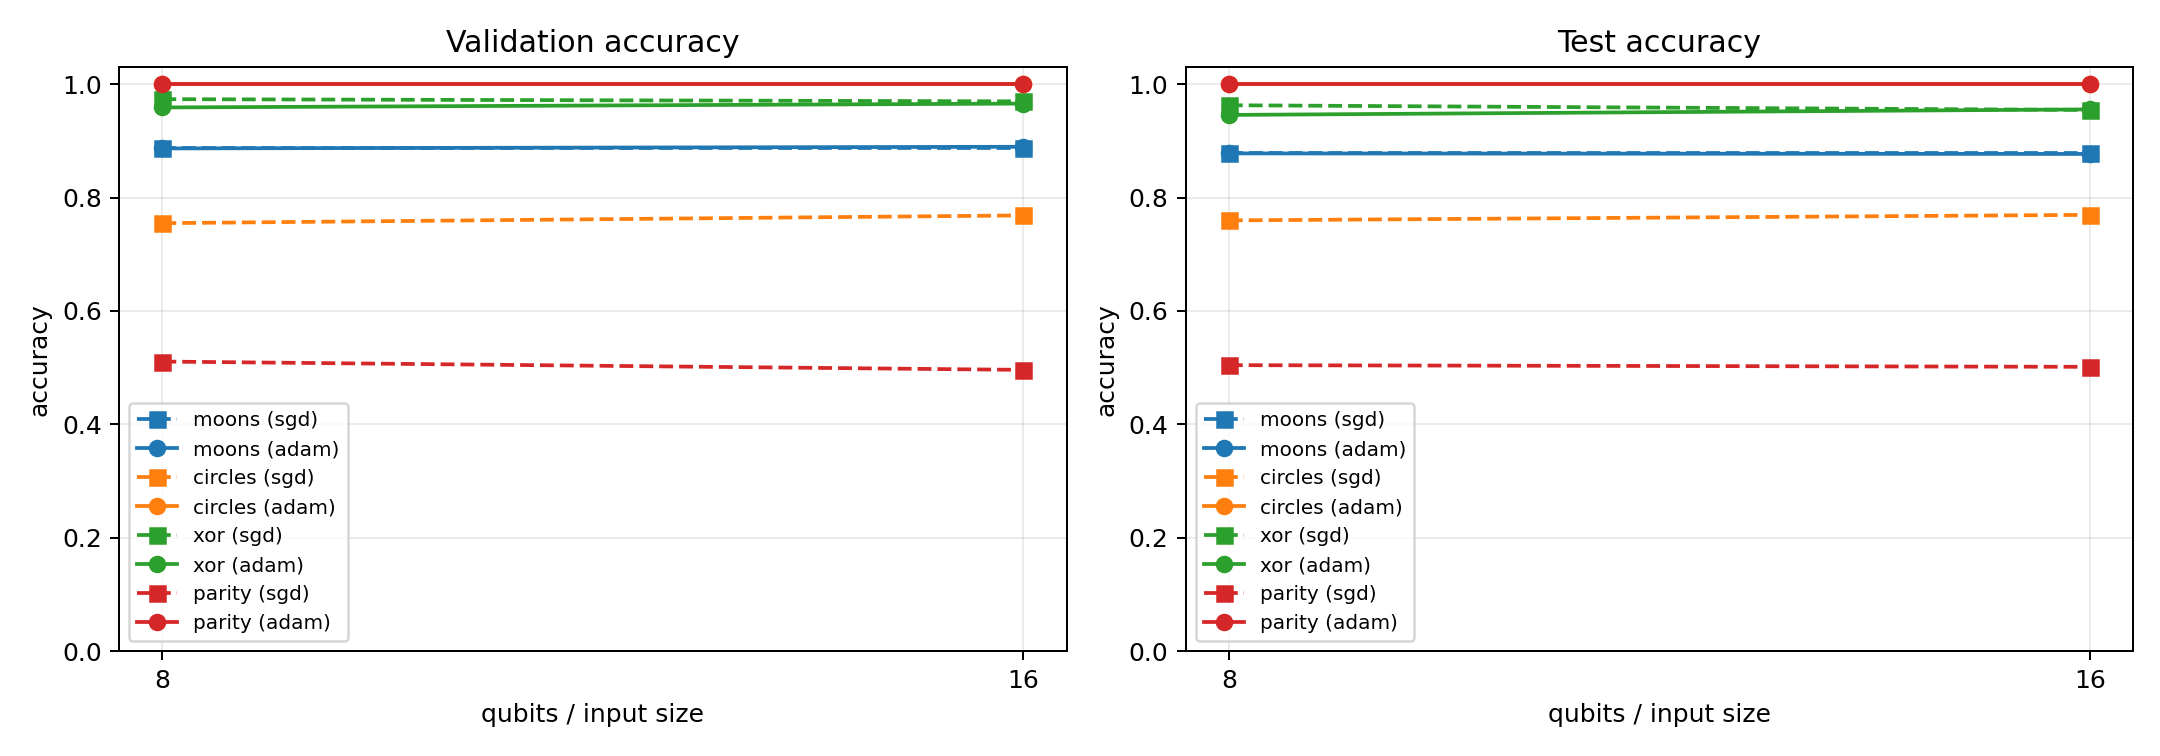
\includegraphics[width=0.90\textwidth]{synthetic_trainability_accuracy.png}
\caption{Validation and test accuracy for the best repeat of each synthetic fixed-information benchmark.}
\end{figure}

\begin{figure}[h]
\centering
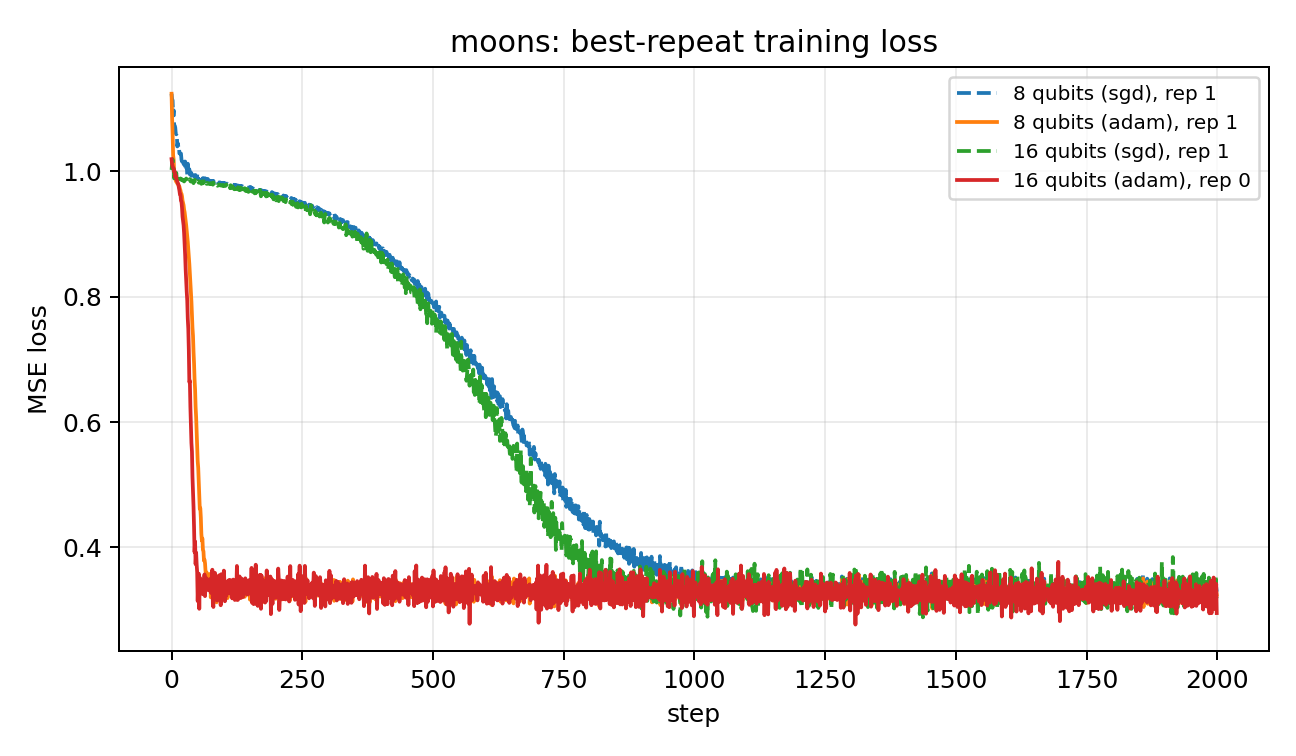
\includegraphics[width=0.72\textwidth]{synthetic_trainability_loss_moons.png}
\caption{Moons benchmark: best-repeat training loss curves.}
\end{figure}

\begin{figure}[h]
\centering
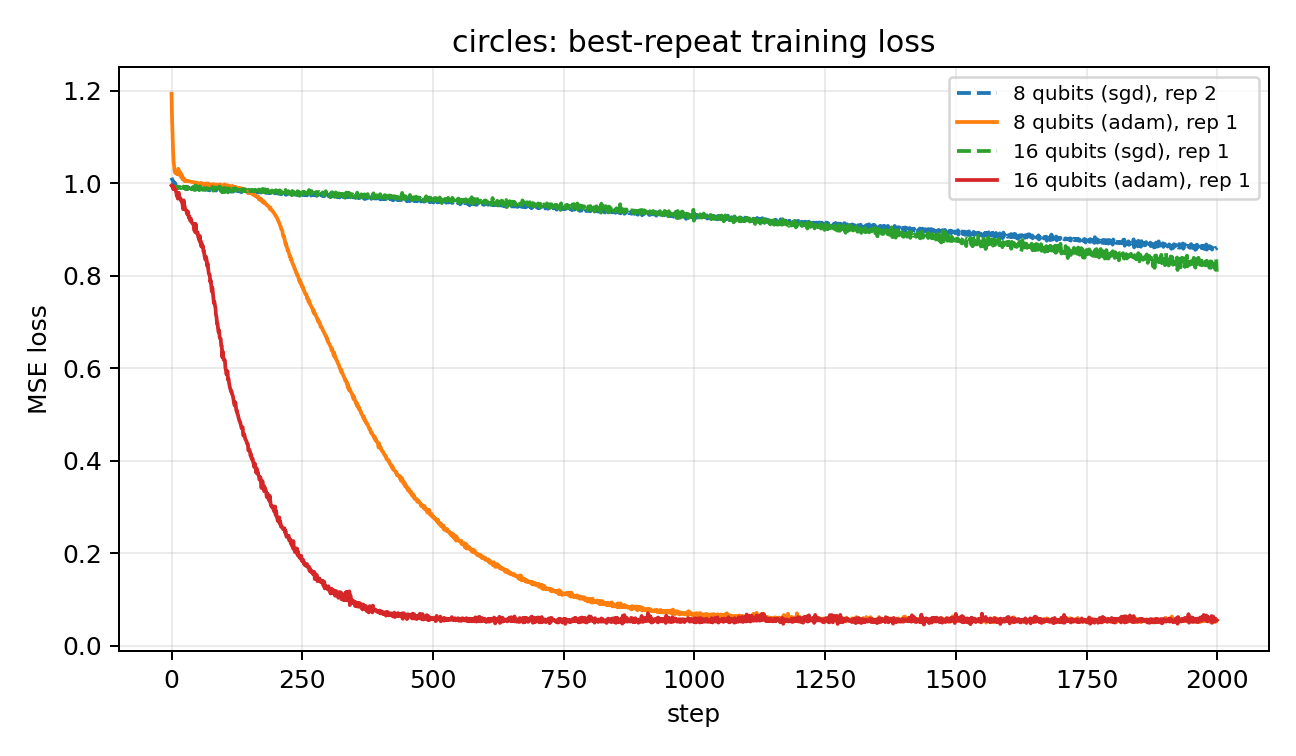
\includegraphics[width=0.72\textwidth]{synthetic_trainability_loss_circles.png}
\caption{Circles benchmark: best-repeat training loss curves.}
\end{figure}

\begin{figure}[h]
\centering
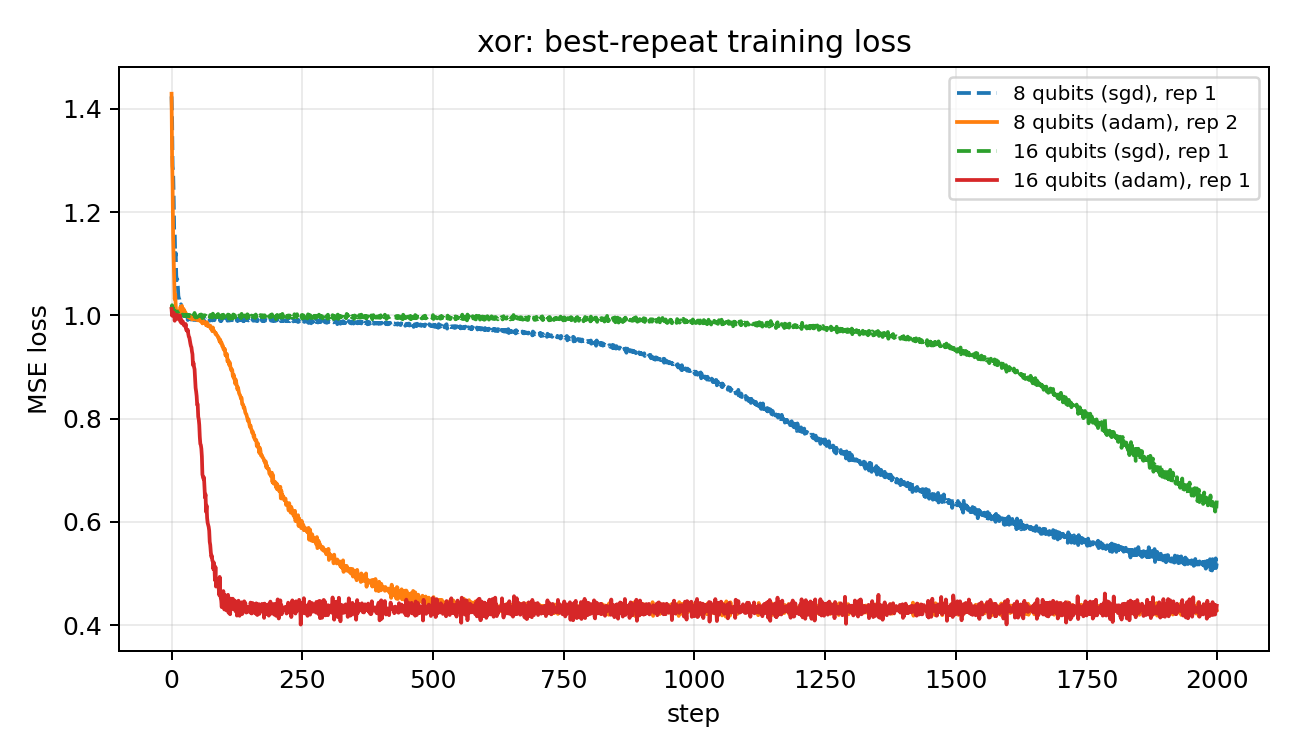
\includegraphics[width=0.72\textwidth]{synthetic_trainability_loss_xor.png}
\caption{XOR benchmark: best-repeat training loss curves.}
\end{figure}

\begin{figure}[h]
\centering
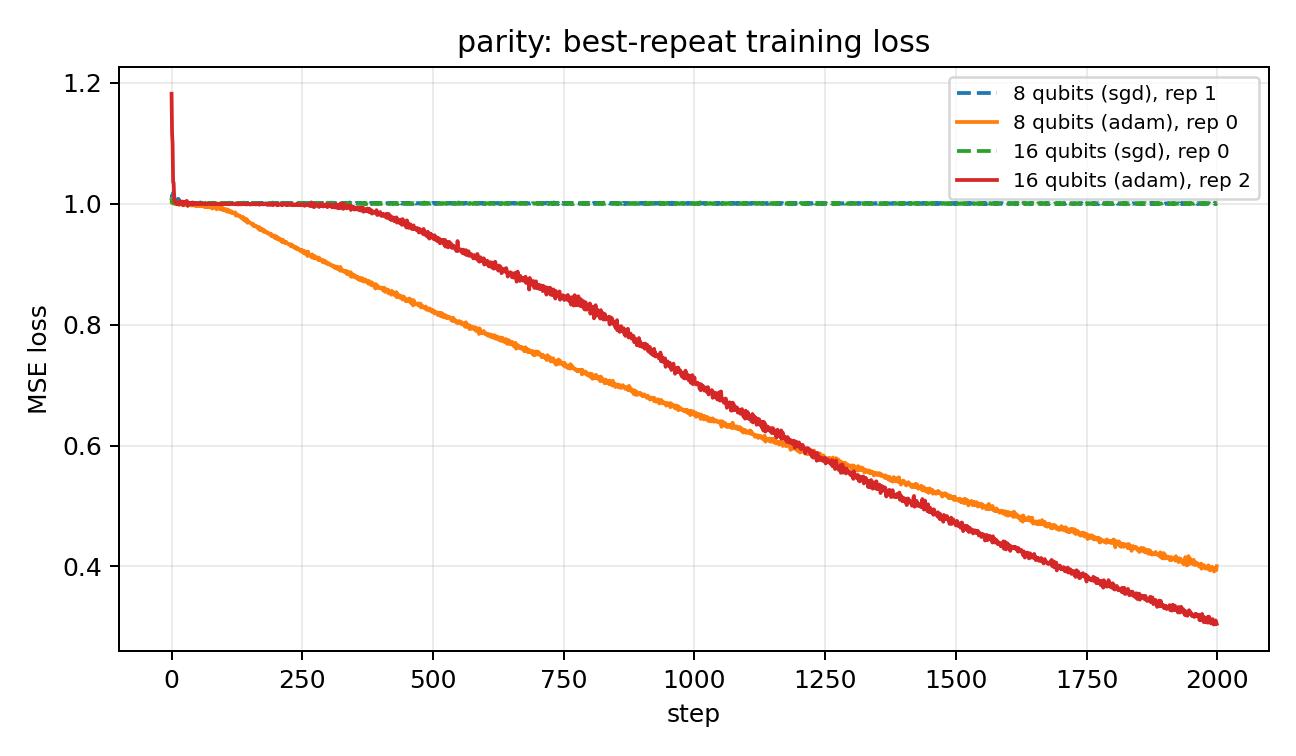
\includegraphics[width=0.72\textwidth]{synthetic_trainability_loss_parity.png}
\caption{Parity benchmark: best-repeat training loss curves.}
\end{figure}

The main qualitative observation is that BMERA is trainable on these small
fixed-information tasks, but optimizer choice matters. Adam reliably solves the
circles and parity tasks and reaches competitive performance on moons and XOR,
while plain SGD fails on parity and is weaker on circles. Increasing from 8 to
16 qubits does not materially improve accuracy in this fixed-information setup,
which is expected because the additional input dimensions are exactly zero
padded. These runs therefore serve primarily as a trainability sanity check, not
as evidence that larger \(N\) improves generalization on fixed low-dimensional
classical data.

\FloatBarrier

\section*{Potential for further improvement}

There is still room to improve, but the next gains should be targeted carefully.
The plots show that throughput peaks before the largest tested batch for
8, 16, and 64 qubits. For 32, 128, and 256 qubits the peak occurs at the largest
successful batch in the current data, so these cases are the strongest candidates
for additional larger-batch or microbatch sweeps.

The highest-priority follow-up is to benchmark fixed microbatch variants instead
of only increasing the full logical batch. For example, sweeps with microbatch
sizes \(64\), \(128\), and \(256\) can test whether logical batches beyond the
current successful points remain stable without increasing the peak live
activation footprint. This should mainly improve maximum stable logical batch,
not necessarily raw throughput.

For throughput, the remaining bottleneck is likely still contraction
materialization and backward-pass residual storage rather than the explicit BMERA
cache itself. The next software targets are a custom VJP around the density-block
contraction, selective rematerialization/checkpointing only at stable contraction
boundaries, and eventually a fused CUDA/C++ kernel for the local
\(U\rho U^\dagger\) block update if profiling confirms that XLA is still creating
large temporaries. Native code is therefore plausible, but the updated results
suggest one more JAX profiling/tuning pass is worthwhile before adding a custom
build system.

\section*{Sources}

\sloppy
\begin{itemize}
  \item NVIDIA GeForce RTX 5070 family specifications:
  \url{https://www.nvidia.com/it-it/geforce/graphics-cards/50-series/rtx-5070-family/}
  \item PCBench GeForce RTX 5070 specification page:
  \url{https://pcbench.net/graphics-cards/nvidia-geforce-rtx-5070}
\end{itemize}

\end{document}
